\documentclass[tikz,border=2pt]{standalone}
\usepackage{amsmath}
\usepackage{pgfplots}
\pgfplotsset{compat=1.18}
\usetikzlibrary{arrows.meta}
\begin{document}
% The four example plots: scatter of Transport vs Buildings (22,20) (24,21) (146,110) (148,115) (30,25) (31,24);
% lines Belgium 25 22 24 and Netherlands 33 29 30 for 2019-2021; histogram of 20 wages, bins of width 5
% from 10 to 45 with counts 3 5 5 3 2 1 1; box plots: degree 18 | 22 24 27.5 | 29 and outlier 45, no degree 12 | 14.5 17 18.5 | 22.
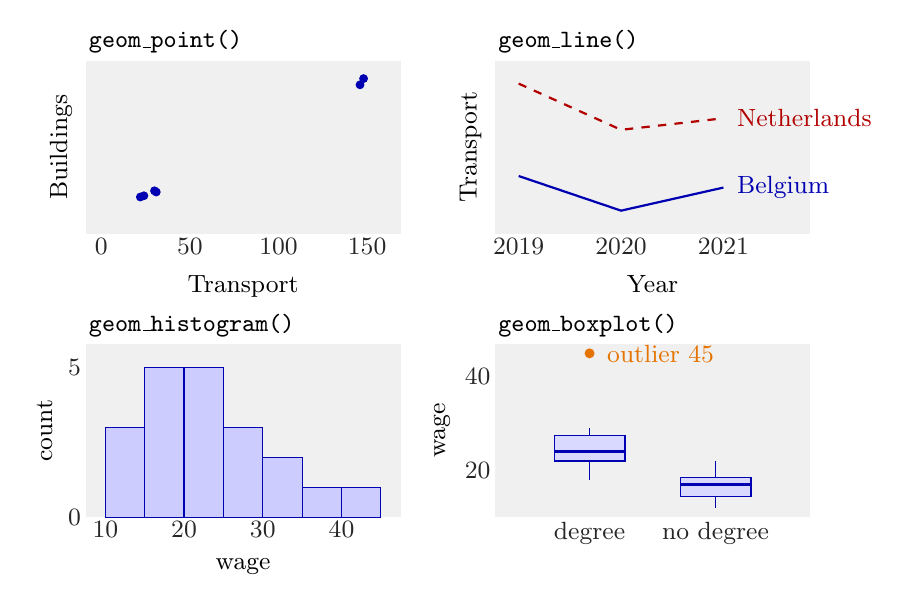
\begin{tikzpicture}[font=\small, >={Latex[length=2mm]},
  code/.style={font=\small\ttfamily, inner sep=1pt},
  tick/.style={gray!30!black, inner sep=1.5pt}]
  \def\pw{4.0}
  \def\ph{2.2}
  % ---------- scatter ----------
  \begin{scope}[shift={(0,3.6)}]
    \fill[gray!12] (0,0) rectangle (\pw,\ph);
    % x 0..160 -> 0.2..3.8, y 0..120 -> 0.15..2.05
    \foreach \a/\b in {22/20,24/21,146/110,148/115,30/25,31/24}
      \fill[blue!70!black] ({0.2+\a*3.6/160},{0.15+\b*1.9/120}) circle (1.6pt);
    \foreach \a in {0,50,100,150} \node[tick, anchor=north] at ({0.2+\a*3.6/160},0) {\a};
    \node[anchor=north] at (0.5*\pw,-0.4) {Transport};
    \node[rotate=90, anchor=south] at (-0.05,0.5*\ph) {Buildings};
    \node[code, anchor=south west] at (0,\ph+0.05) {geom\_point()};
  \end{scope}
  % ---------- lines ----------
  \begin{scope}[shift={(5.2,3.6)}]
    \fill[gray!12] (0,0) rectangle (\pw,\ph);
    % x 2019..2021 -> 0.3..2.9, y 20..35 -> 0..\ph
    \draw[blue!70!black, thick] (0.3,{(25-20)*\ph/15}) -- (1.6,{(22-20)*\ph/15}) -- (2.9,{(24-20)*\ph/15});
    \draw[red!70!black, thick, dashed] (0.3,{(33-20)*\ph/15}) -- (1.6,{(29-20)*\ph/15}) -- (2.9,{(30-20)*\ph/15});
    \node[blue!70!black, anchor=west] at (2.95,{(24-20)*\ph/15}) {Belgium};
    \node[red!70!black, anchor=west] at (2.95,{(30-20)*\ph/15}) {Netherlands};
    \foreach \x/\t in {0.3/2019,1.6/2020,2.9/2021} \node[tick, anchor=north] at (\x,0) {\t};
    \node[anchor=north] at (0.5*\pw,-0.4) {Year};
    \node[rotate=90, anchor=south] at (-0.05,0.5*\ph) {Transport};
    \node[code, anchor=south west] at (0,\ph+0.05) {geom\_line()};
  \end{scope}
  % ---------- histogram ----------
  \begin{scope}[shift={(0,0)}]
    \fill[gray!12] (0,0) rectangle (\pw,\ph);
    % x 10..45 -> 0.25..3.75 (0.1 per unit), y 0..5 -> 0..1.9
    \foreach \c [count=\i from 0] in {3,5,5,3,2,1,1}
      \draw[blue!70!black, fill=blue!20] ({0.25+\i*0.5},0) rectangle ({0.75+\i*0.5},{\c*1.9/5});
    \foreach \x in {10,20,30,40} \node[tick, anchor=north] at ({0.25+(\x-10)*0.1},0) {\x};
    \foreach \y in {0,5} \node[tick, anchor=east] at (0,{\y*1.9/5}) {\y};
    \node[anchor=north] at (0.5*\pw,-0.4) {wage};
    \node[rotate=90, anchor=south] at (-0.3,0.5*\ph) {count};
    \node[code, anchor=south west] at (0,\ph+0.05) {geom\_histogram()};
  \end{scope}
  % ---------- box plots ----------
  \begin{scope}[shift={(5.2,0)}]
    \fill[gray!12] (0,0) rectangle (\pw,\ph);
    % y 10..47 -> 0..\ph
    \foreach \x/\lo/\qa/\me/\qb/\hi in {1.2/18/22/24/27.5/29, 2.8/12/14.5/17/18.5/22} {
      \draw[blue!70!black] (\x,{(\lo-10)*\ph/37}) -- (\x,{(\qa-10)*\ph/37});
      \draw[blue!70!black] (\x,{(\qb-10)*\ph/37}) -- (\x,{(\hi-10)*\ph/37});
      \draw[blue!70!black, fill=blue!15] (\x-0.45,{(\qa-10)*\ph/37}) rectangle (\x+0.45,{(\qb-10)*\ph/37});
      \draw[blue!70!black, very thick] (\x-0.45,{(\me-10)*\ph/37}) -- (\x+0.45,{(\me-10)*\ph/37});
    }
    \fill[orange!90!black] (1.2,{(45-10)*\ph/37}) circle (1.8pt);
    \node[orange!90!black, anchor=west] at (1.3,{(45-10)*\ph/37}) {outlier 45};
    \node[tick, anchor=north] at (1.2,0) {degree};
    \node[tick, anchor=north] at (2.8,0) {no degree};
    \foreach \y in {20,40} \node[tick, anchor=east] at (0,{(\y-10)*\ph/37}) {\y};
    \node[rotate=90, anchor=south] at (-0.45,0.5*\ph) {wage};
    \node[code, anchor=south west] at (0,\ph+0.05) {geom\_boxplot()};
  \end{scope}
\end{tikzpicture}
\end{document}
